\documentclass[conference]{IEEEtran}
\IEEEoverridecommandlockouts
% The preceding line is only needed to identify funding in the first footnote. If that is unneeded, please comment it out.
\usepackage{cite}
\usepackage{amsmath,amssymb,amsfonts}
\usepackage{algorithmic}
\usepackage{graphicx}
\usepackage{textcomp}
\usepackage{xcolor}
\usepackage{subcaption}
\def\BibTeX{{\rm B\kern-.05em{\sc i\kern-.025em b}\kern-.08em
    T\kern-.1667em\lower.7ex\hbox{E}\kern-.125emX}}
\begin{document}

\title{UVM and SVA Based Functional Verification of an SLM Wear-out Monitoring IP}

\author{\IEEEauthorblockN{Shidi Xi}
\IEEEauthorblockA{\textit{Department of Electrical and Computer Engineering} \\
\textit{The University of British Columbia}\\
Vancouver V6T 1Z4, Canada \\
xsd99@ece.ubc.ca}
}

\maketitle

\begin{abstract}
    Nowadays, many SLM IPs are being integrated into SoCs, and effective functional verification of them is becoming increasingly important. Meanwhile, on-chip communication interfaces are also growing more complex. As an essential component of any SoC IP, this puts additional demands on the IP's verification process. In this report, an SLM wear-out monitoring IP with an AMBA APB interface has been verified using UVM and SVA. UVM testbenches capable of generating constrained random stimuli were developed for different levels of the design, and SVA properties were written for the APB interface. 100\% functional coverage has been achieved, demonstrating the effectiveness of the methodology.
 \end{abstract}
 
 %\begin{IEEEkeywords}
 %    UVM, SVA, Verification, APB
 %\end{IEEEkeywords}
 
 \section{Introduction}
 Universal Verification Methodology (UVM) is a standardized methodology for functional coverage-driven verification of digital designs, primarily in SystemVerilog \cite{UVM}. It enables the creation of reusable, modular, and scalable testbenches, making it a dominant choice in the IC verification industry. SystemVerilog Assertions (SVA) is an integral part of the SystemVerilog language that provides a well-structured way of integrating assertions into testbenches written in SystemVerilog \cite{SV}. SVA can be used to check the temporal and functional properties of the design under test (DUT) and are particularly useful when verifying a communication protocol such as AMBA APB.
 
 Silicon life management (SLM) involves techniques to monitor, predict, and extend the operational life of ICs. It is critical in industries where circuit reliability is a top concern, such as automotive, biomedical, and aerospace \cite{Hill2024}. One aspect of SLM is wear-out monitoring, which involves using on-chip sensors to constantly measure the physical and electrical characteristics of an IC to detect signs of circuit degradation (wear-out) caused by wear-out mechanisms. Common parameters to monitor include voltage, temperature, and frequency. Common wear-out mechanisms include bias threshold instability (BTI), hot carrier injection (HCI), electromigration (EM), and stress-induced leakage current (SILC). 
 
 A wear-out monitoring IP can be used within a system-on-chip (SoC) to gather on-chip sensor readings and transfer the data back to the CPU. Usually, the IP contains logic to collect and analyze output from ADCs, which digitalize the sensors' analog output. Its communication with the CPU is typically enabled by a standard on-chip bus protocol such as AMBA APB. APB is part of the AMBA protocol family, designed to bridge low-speed and low-power peripherals to the processor.
 
 This report presents the verification methodology and results of an SLM wear-out monitoring IP designed in-house. Using UVM and SVA, the functionality of the IP and its APB interface have been successfully verified with full functional coverage. An overview of the IP and the APB protocol is presented in Section II. Section III describes the verification strategy, followed by the UVM testbench architecture and SVA properties in Section IIII and V. Section VI presents the verification results and Section VII concludes the report.
 
\section{DUT Overview}
\subsection{IP Functionalities}
Figure \ref{fig:dut} presents the IP's block diagram. The IP, depicted by the yellow block, consists of data processing modules on the right to gather and analyze the data from the on-chip wear-out sensors. The IP also has an APB interface to enable communication with the CPU. In addition, there are some internal registers within the IP. The CPU Commands Register takes in commands from the CPU through APB. These commands control the sensor modules to provide data back to the CPU, which will be written into the Sensor Measurement Register before being sent out on the APB interface.  
 
\begin{figure}[h!]
    \centering
    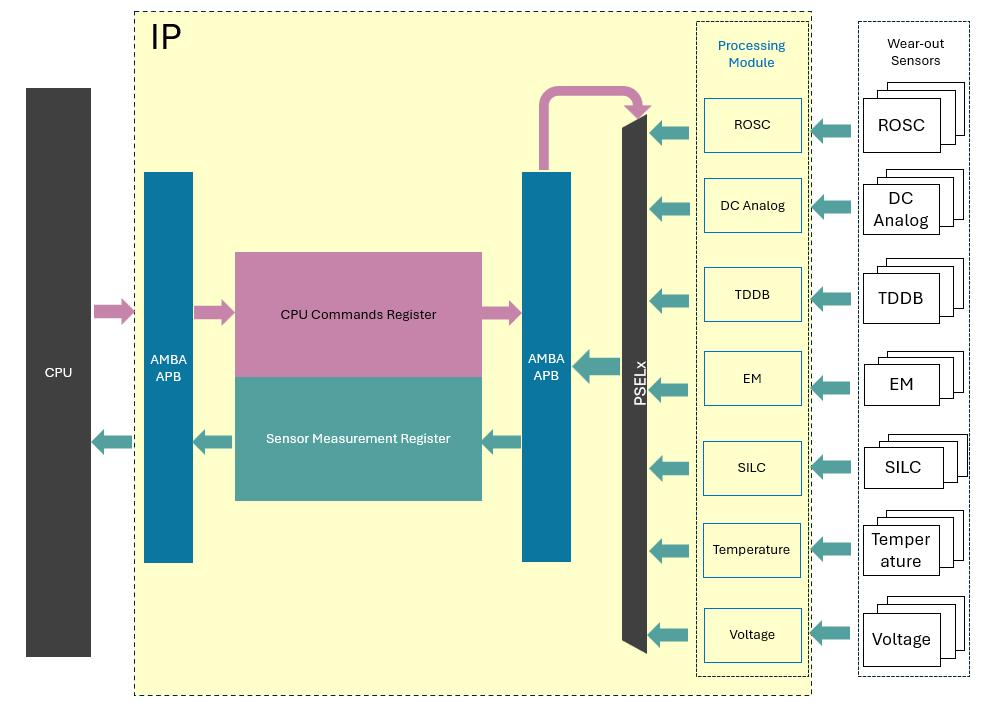
\includegraphics[width = 0.5\textwidth]{figures/dut.jpg}
    \caption{Block diagram of the SLM wear-out monitoring IP \cite{Peng2024}.}
    \label{fig:dut}
\end{figure}
\subsection{AMBA APB Protocol}
APB is a low-cost and easy-to-implement interface protocol that is commonly used to enable data transfer between the CPU and on-chip low-power peripherals \cite{APB}. In the protocol, a requester, usually the CPU, requests data from a completer, who responds to the request with data. Oftentimes, the peripherals serve the role of the completers. Both parties must have the same set of interface signals defined by the protocol. Some of the essential signals of APB are listed in Table \ref{tab:apb}.

\begin{table}[h!]
    \caption{List of core signals of the APB interface \cite{APB}.}
    \centering
    \begin{tabular}{|c c c c|}
        \hline
        Signal & Source & Width & Description \\
        \hline
        PCLK & Clock & 1 & Clock signal. \\
        PADDR & Requester & ADDR\_WIDTH & APB address bus. \\
        PSEL & Requester & 1 & Select.  \\
        PENABLE & Requester & 1 & Enable. \\
        PWRITE & Requester & 1 & Direction. \\ 
        PWDATA & Requester & DATA\_WIDTH & Write data. \\
        PREADY & Completer & 1 & Transaction complete. \\
        PRDATA & Completer & DATA\_WIDTH & Read data. \\
        \hline  
    \end{tabular}
    \label{tab:apb}
\end{table}

Figure \ref{fig:apb_write} illustrates an APB write transfer. At T1, the requester asserts PSEL to select a completer. PADDR, PWRITE, and PWDATA must be valid at the same time (PWRITE is high during write). Then at T2, PENABLE is asserted, signaling the start of a transaction. All the signals mentioned above must be stable until the completer asserts PREADY at T4, indicating that PWDATA will be accepted at the next cycle. Lastly, at T5, PSEL and PENABLE must be deasserted to finish the transaction.

\begin{figure}[h!]
    \centering
    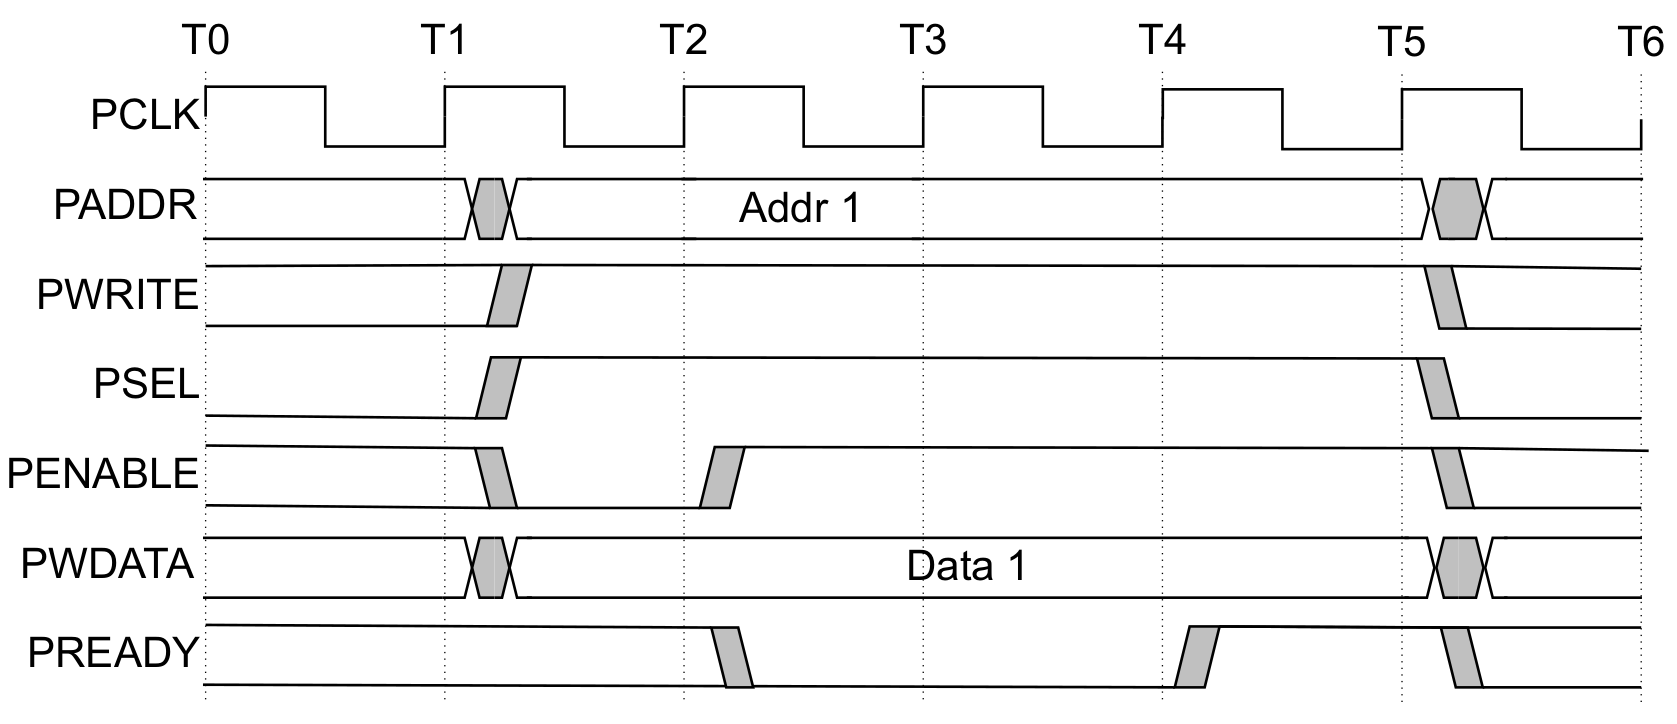
\includegraphics[width = 0.4\textwidth]{figures/apb_write.png}
    \caption{APB write transfer \cite{APB}.}
    \label{fig:apb_write}
\end{figure}

Figure \ref{fig:apb_read} illustrates an APB read transfer. The timing of PADDR, PWRITE, PSEL, and PENABLE are the same as the write operation. Notice PWRITE must be low when reading, and when the completer has the valid data, it must drive it on PRDATA and assert PREADY at the same time.

\begin{figure}[h!]
    \centering
    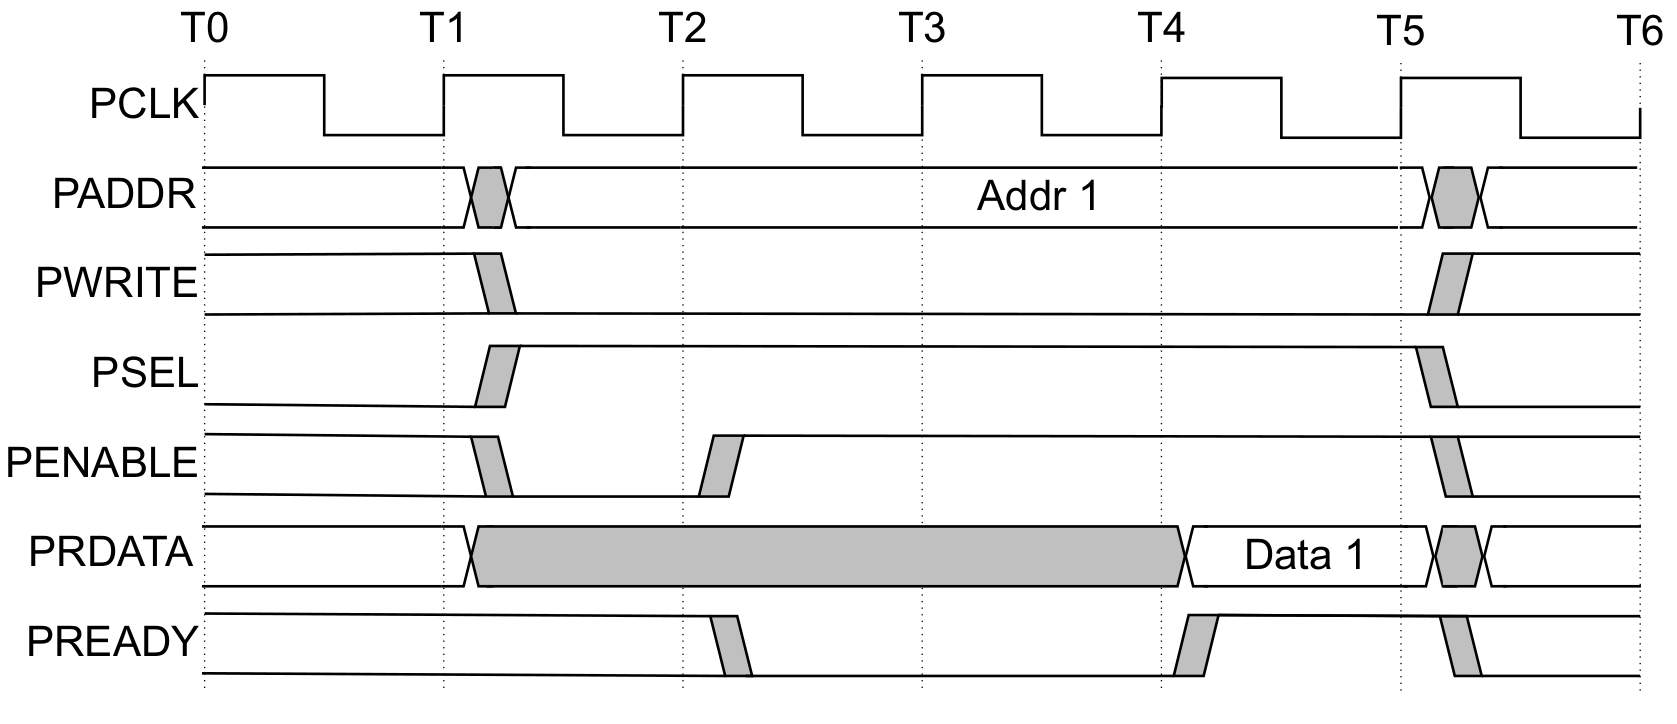
\includegraphics[width = 0.4\textwidth]{figures/apb_read.png}
    \caption{APB read transfer \cite{APB}.}
    \label{fig:apb_read}
\end{figure}

\section{Verification Strategy}
The verification strategy was developed alongside the RTL design of the IP, employing a bottom-up approach to match the design's development. The IP's individual sensor processing modules were designed first, followed by their integration into the IP along with the APB interface. Consequently, the verification process consisted of three distinct stages:

\begin{itemize}
    \item \textbf{Module level}: Verified the functionalities of individual modules as they were developed. Each module had its own UVM testbench, coverpoints, and test cases.
    \item \textbf{IP level}: Conducted full IP verification after integrating all components. A separate testbench was created, combining coverpoints and test cases from individual modules.
    \item \textbf{APB interface}: Ensured that the APB interface adhered to the protocol. SVA was employed for this purpose instead of UVM.
\end{itemize}

\section{UVM Testbench Architecture}

The UVM framework consists of several components that form a structured testbench architecture. Each component, with a unique functionality, is a self-contained class implemented using object-oriented programming (OOP) in SystemVerilog, making them easily reusable across different testbenches or projects. Figure \ref{fig:uvm} shows a standard architecture of a UVM testbench containing all the common components.


\begin{figure}[h!]
    \centering
    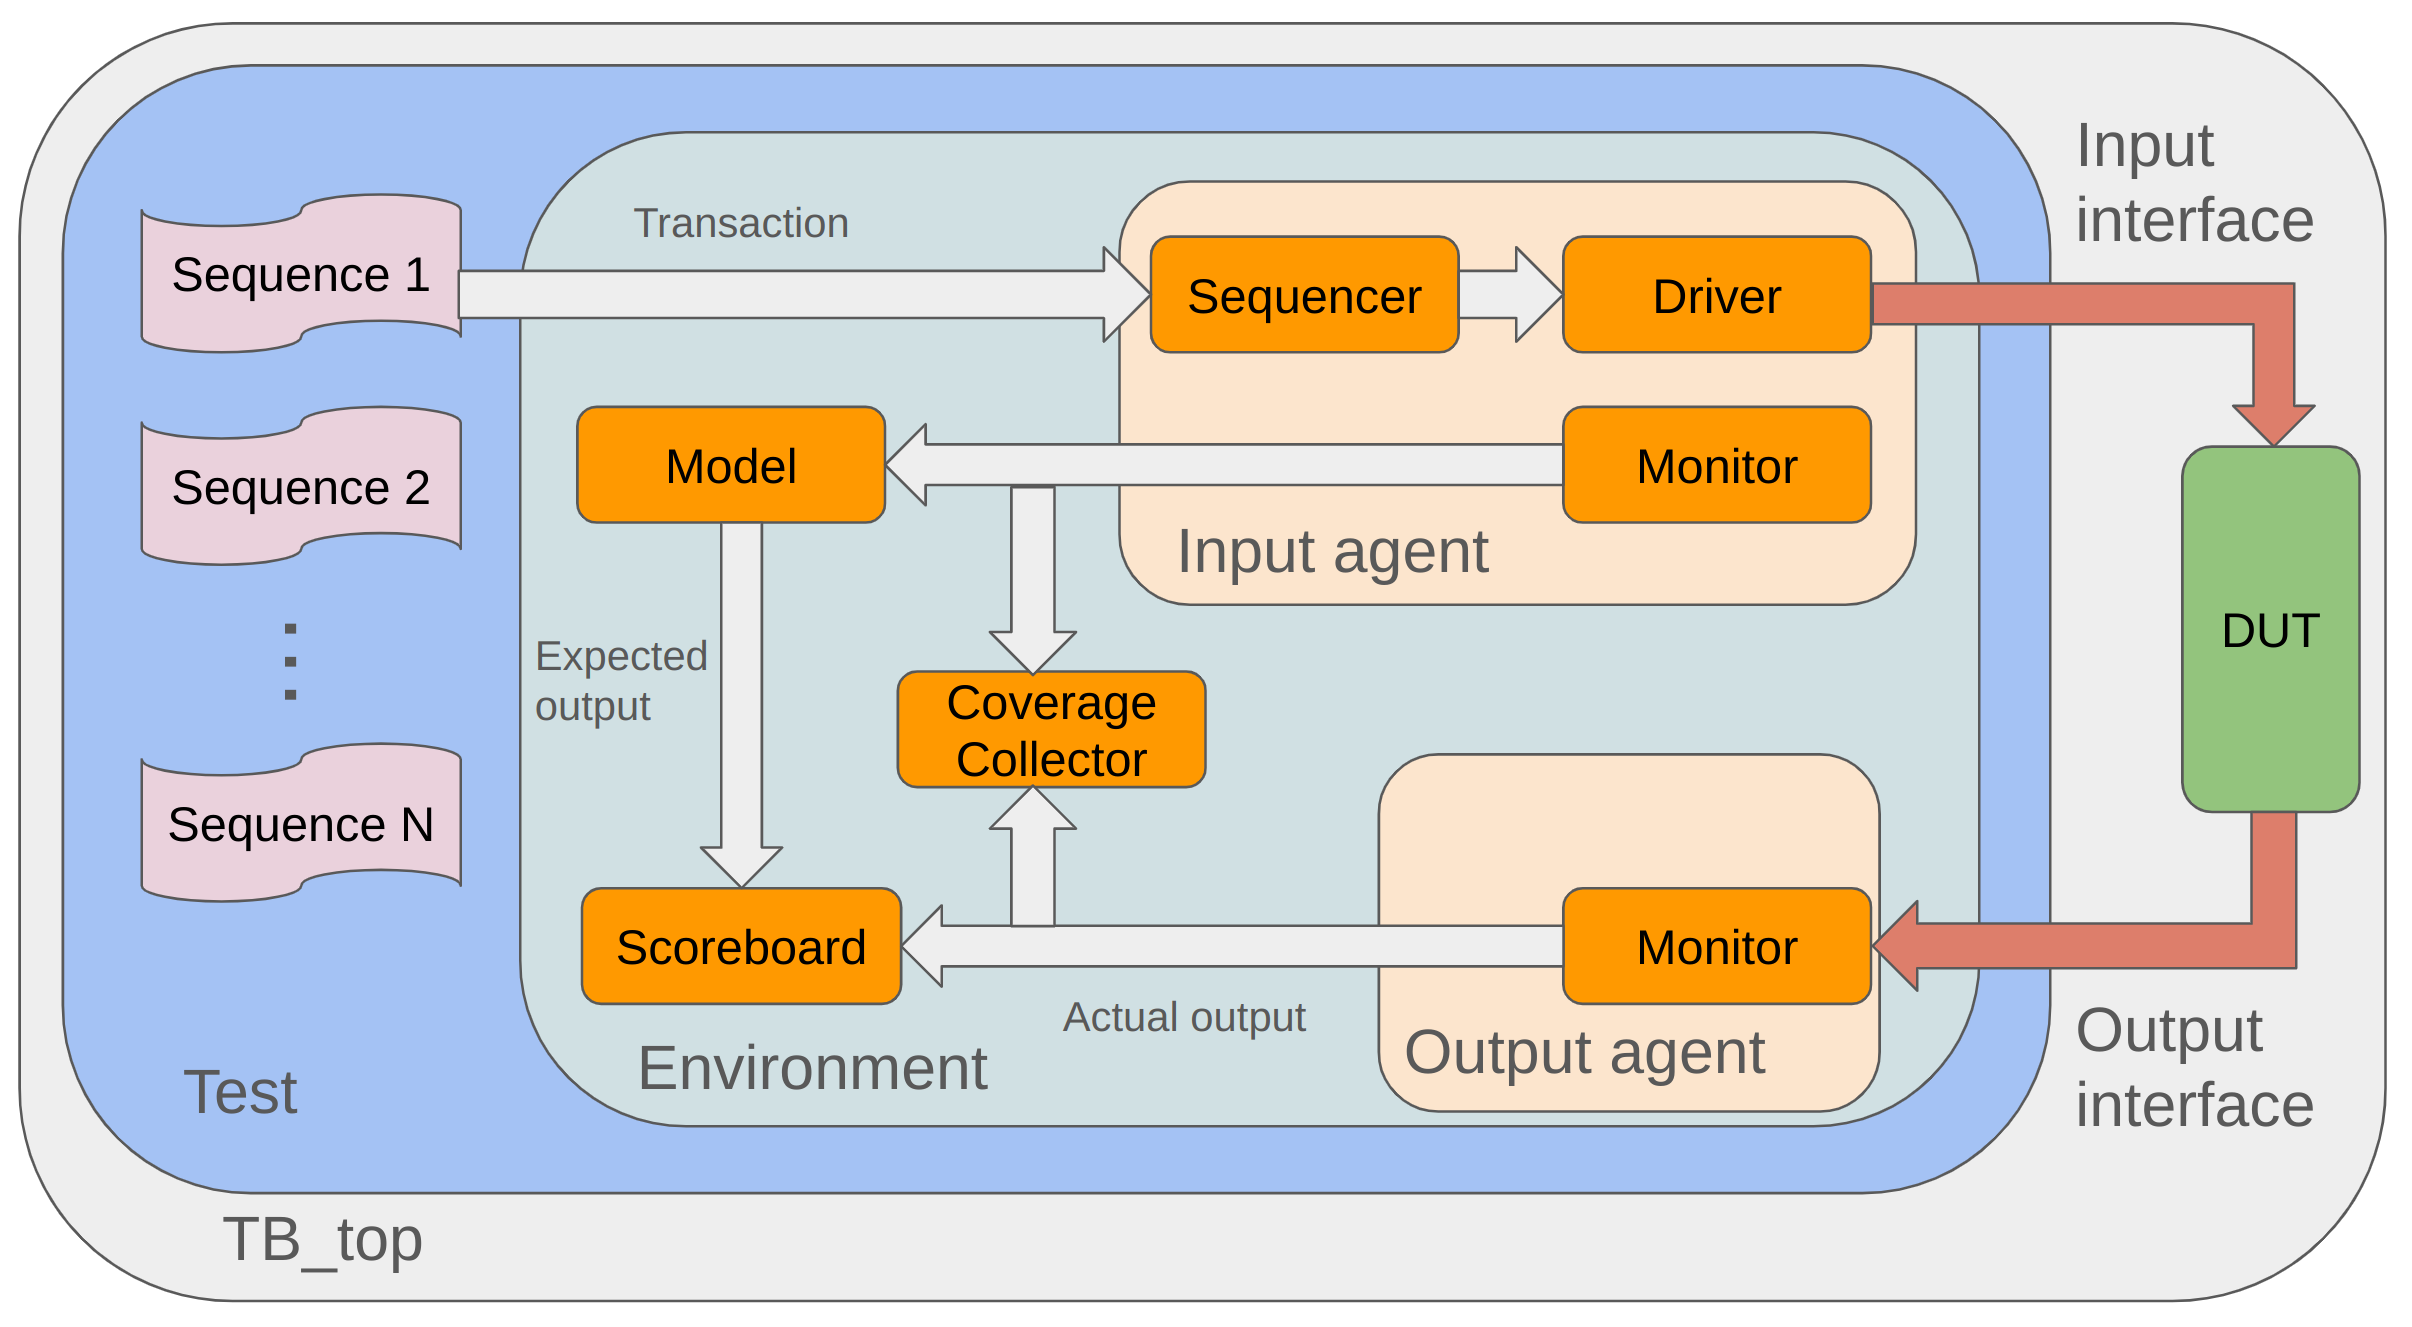
\includegraphics[width = 0.5\textwidth]{figures/uvm.png}
    \caption{UVM testbench architecture.}
    \label{fig:uvm}
\end{figure}

\begin{itemize}
    \item \textbf{TB\_top}: The top module of the testbench, not a UVM component. It instantiates a Test object, the DUT, and two interfaces positioned at the input and output, respectively.
    \item \textbf{Test}: Instantiates the Environment and several Sequences. It configures the Environment and controls the test flow by sequentially starting the Sequences.
    \item \textbf{Sequence}: Describes the desired stimuli as a series of Transactions. For example, corner case stimuli reside in one Sequence, while error case stimuli are in another. Completion of all Sequences ensures all desired stimuli are applied to the DUT and test cases are covered.
    \item \textbf{Environment}: A container class consisting of Agents, a Model, a Scoreboard, and a Coverage Collector.
    \item \textbf{Agent}: A container class that can be either active or passive. An active Agent, typically at the input, includes a Sequencer, Driver, and Monitor. A passive Agent, usually at the output, contains only a Monitor.
    \item \textbf{Sequencer}: Receives transactions from Sequences and schedules them for the Driver.
    \item \textbf{Driver}: Converts transactions from the Sequencer into pin-level activities and drives the DUT's pins via an interface.
    \item \textbf{Monitor}: Observes pin activities on the interface, transforms them into transaction objects, and sends them to the Model, Scoreboard, or Coverage Collector.
    \item \textbf{Model}: Fully emulates the DUT's behavior, generating the expected output for given inputs and sending it to the Scoreboard.
    \item \textbf{Scoreboard}: Compares the expected output from the Model with the actual output from the DUT.
    \item \textbf{Coverage Collector}: Defines coverpoints for the DUT based on its specifications and collects coverage information from the input and output Agents.
\end{itemize}

Each module in the IP, along with the IP itself, had a dedicated testbench based on the architecture described above. These testbenches differed in their Sequences due to varying functionalities and test cases.

\section{APB Verification by SVA}
Based on the APB protocol described in Section II.B, the following properties must hold during the operation of the IP:

\begin{itemize}
    \item If PENABLE is asserted, it must remain high until PREADY is also asserted.
    \item If PENABLE and PREADY are both high in a given cycle, the transaction must be completed, and PENABLE deasserted in the next cycle.
    \item During a write transaction, while PENABLE is high, PADDR, PWRITE, and PWDATA must remain stable.
    \item During a read transaction, while PENABLE is high, PADDR and PWRITE must remain stable.
\end{itemize}

These properties were implemented using SVA and integrated into the IP's UVM testbench. While the DUT responded to stimuli generated by UVM Sequences and its operation was scrutinized by the Monitor and Scoreboard, these assertions were evaluated in parallel.


\section{Results}
This section presents the simulation waveforms and the coverage report for the IP level verification. All simulations were conducted using Vivado. Figure \ref{fig:report} is the UVM report generated when the simulation had completed. It shows that there is no warning, error, or fatal error during the entire simulation. This indicates that the IP is functionaly correct.

\begin{figure}[h!]
    \centering
    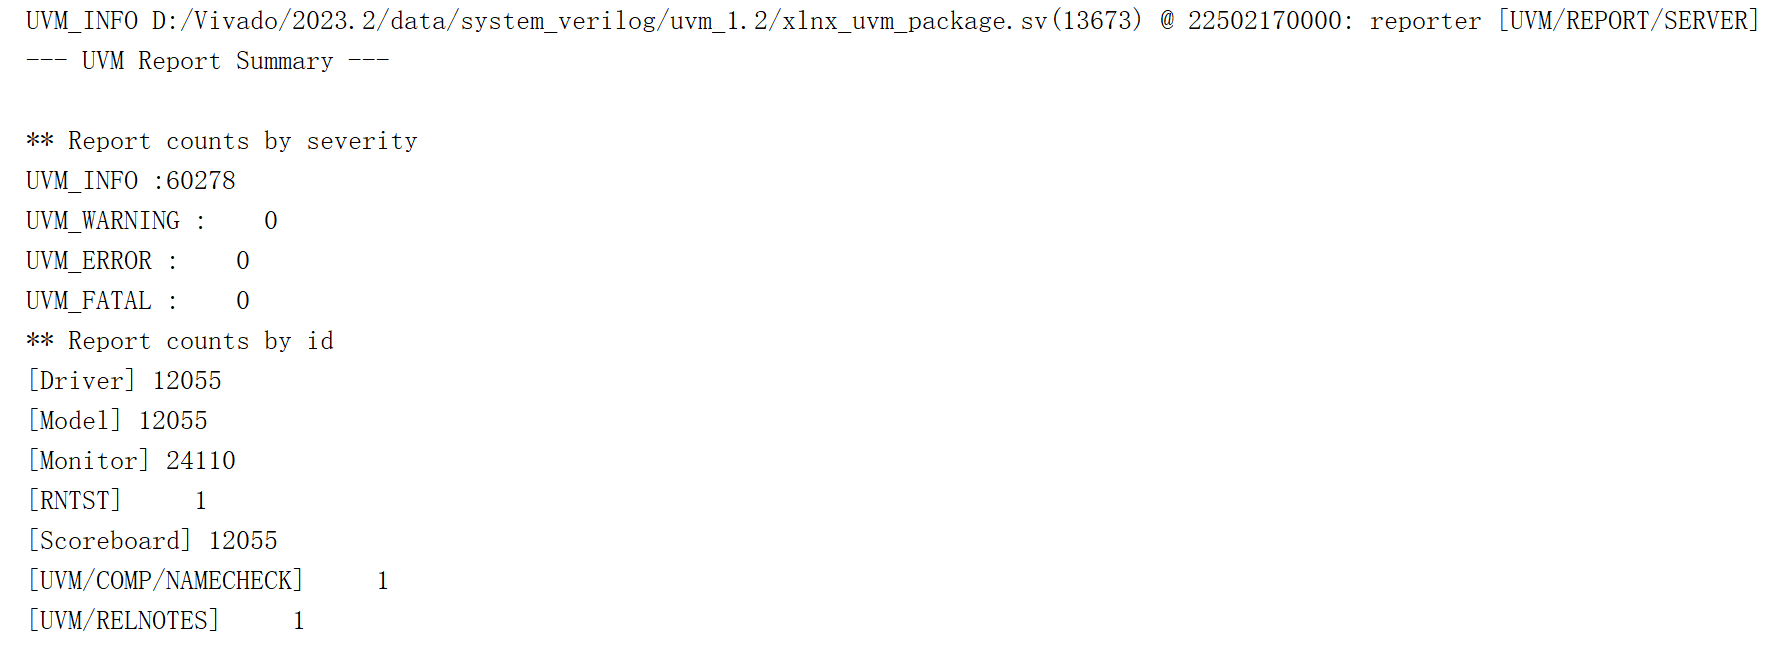
\includegraphics[width = 0.5\textwidth]{figures/report.png}
    \caption{UVM simulation report.}
    \label{fig:report}
\end{figure}

\subsection{Test Case 1: Random Normal Operation}
Figure \ref{fig:random} presents two random transactions between the UVM testbench and the DUT. First, a UVM Sequence generated a random transaction, which was then given to the UVM Sequencer. The Sequencer scheduled the transaction to the UVM Driver. The Driver converted the transaction to pin-activities and drove 'h90723ffc on the CPUCommand bus shown in the figure. At the same time, the UVM Model received the same transaction and produced the expected output for the UVM Scoreboard. Inside the DUT, 'h90723ffc was written into the IP's CPU Commands Register (Figure \ref{fig:dut}) via the APB interface. Then the command activated a particular sensor module (the analog sensor module in this case) which would start gathering data from its corresponding sensor. Eventually, the result, 'h01732001, was written into the Sensor Measurement Register and driven onto the ResultForCPU bus shown in the figure. This output was collected by the UVM Monitor who then sent it to the Scoreboard to compare with the expected output and to the Coverage Collector for coverage measurement. The check passed in the Scoreboard and a new transaction, marked by 'hb032fffc on the CPUCommand bus, was generated. The process repeated until the entire UVM Sequence had been completed.
\begin{figure}[h!]
    \centering
    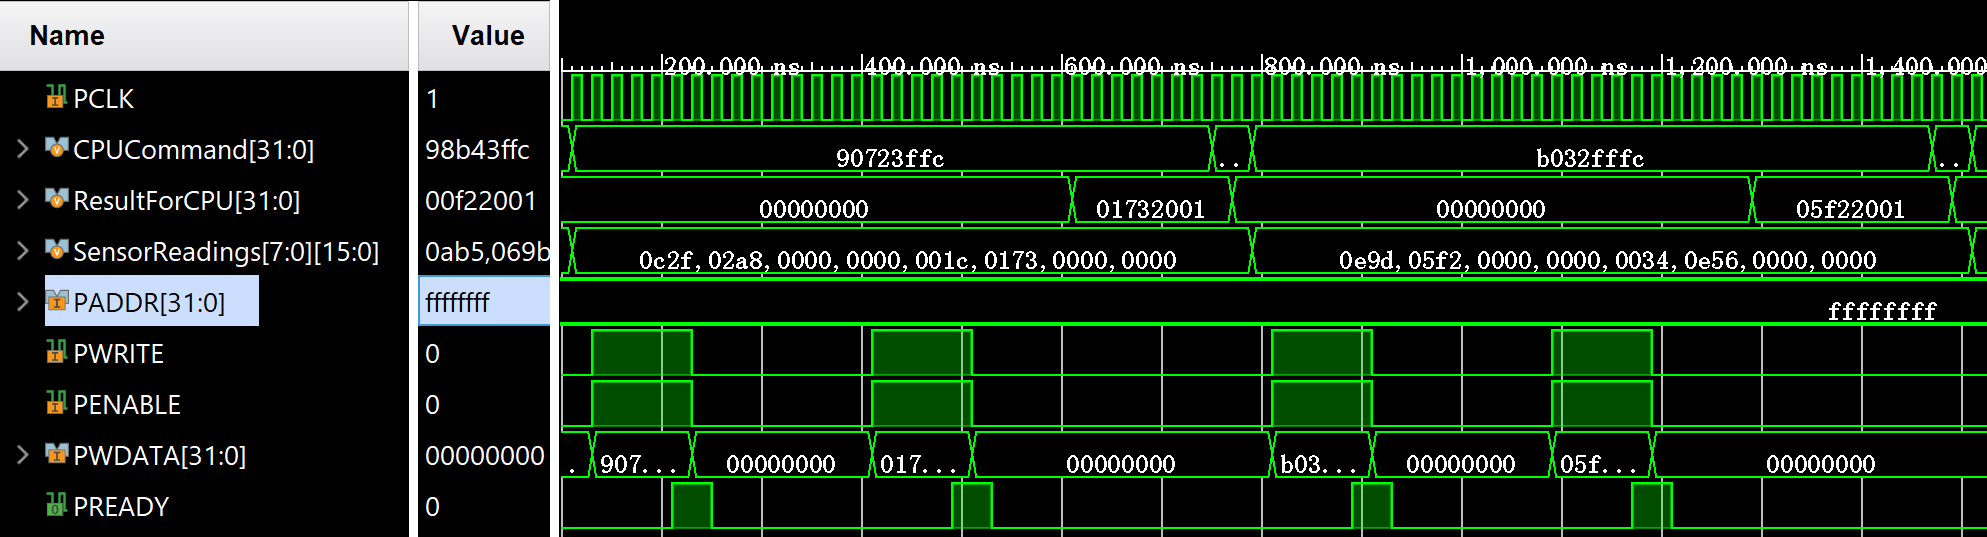
\includegraphics[width = 0.5\textwidth]{figures/random.png}
    \caption{Simulation waveform of random normal operation.}
    \label{fig:random}
\end{figure}

\subsection{Test Case 2: Corner Case}
Figure \ref{fig:corner} shows the waveform of a corner case (0 measurement cycles for the SILC module). This is to demonstrate that UVM Sequences can be constrained to generate direct test cases to cover corner scenarios.

\begin{figure}[h!]
    \centering
    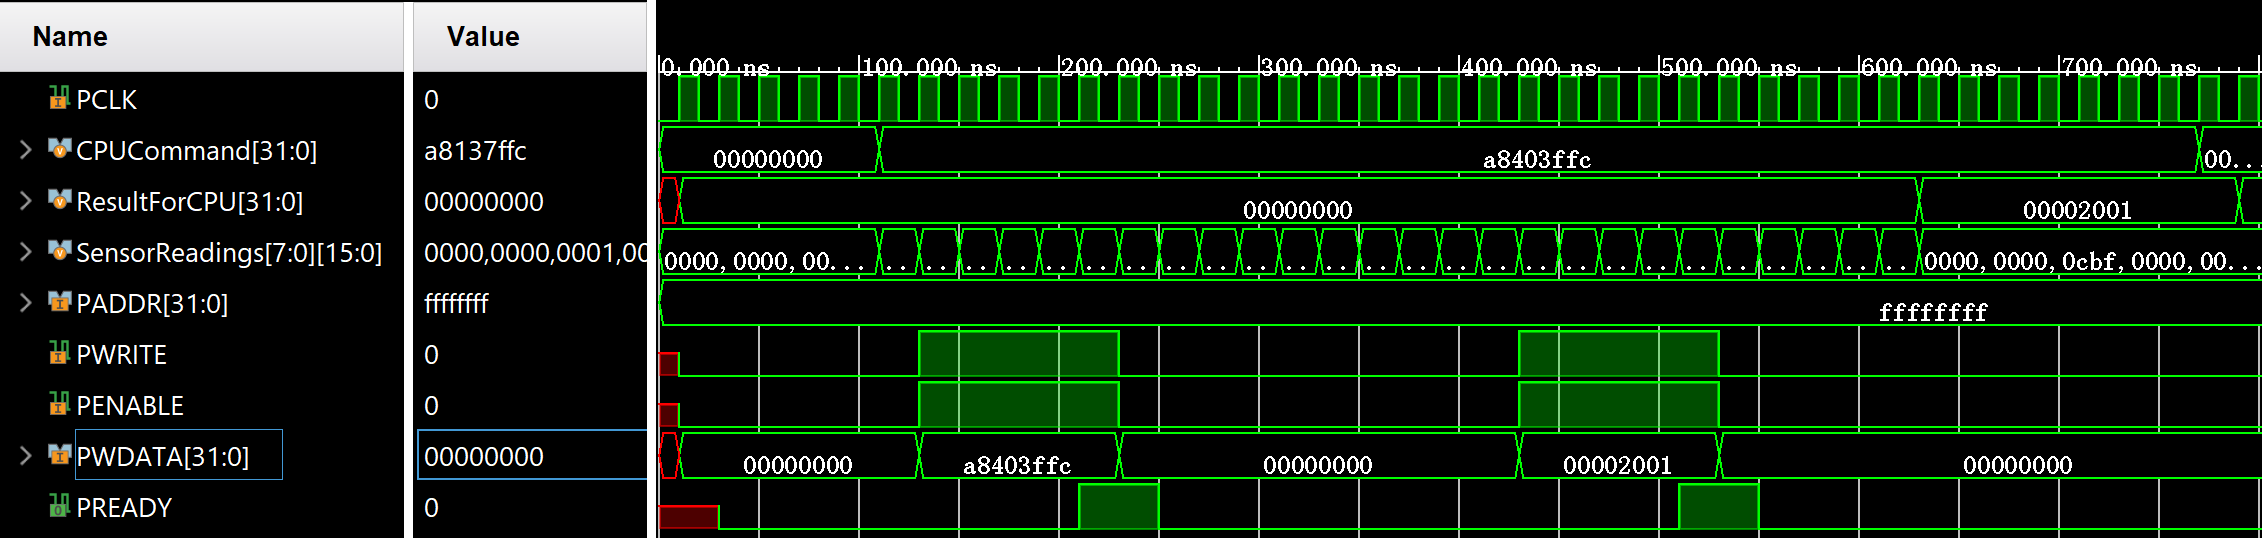
\includegraphics[width = 0.5\textwidth]{figures/corner.png}
    \caption{Simulation waveform of a corner case.}
    \label{fig:corner}
\end{figure}

\subsection{Test Case 3: Error Case}
Figure \ref{fig:error} shows the waveform of an error case (0 threshold for the SILC module). It demonstrates the DUT's behavior under erroneous inputs. The ResultForCPU bus shows 'h000e001 indicating an error has occurred.
\begin{figure}[h!]
    \centering
    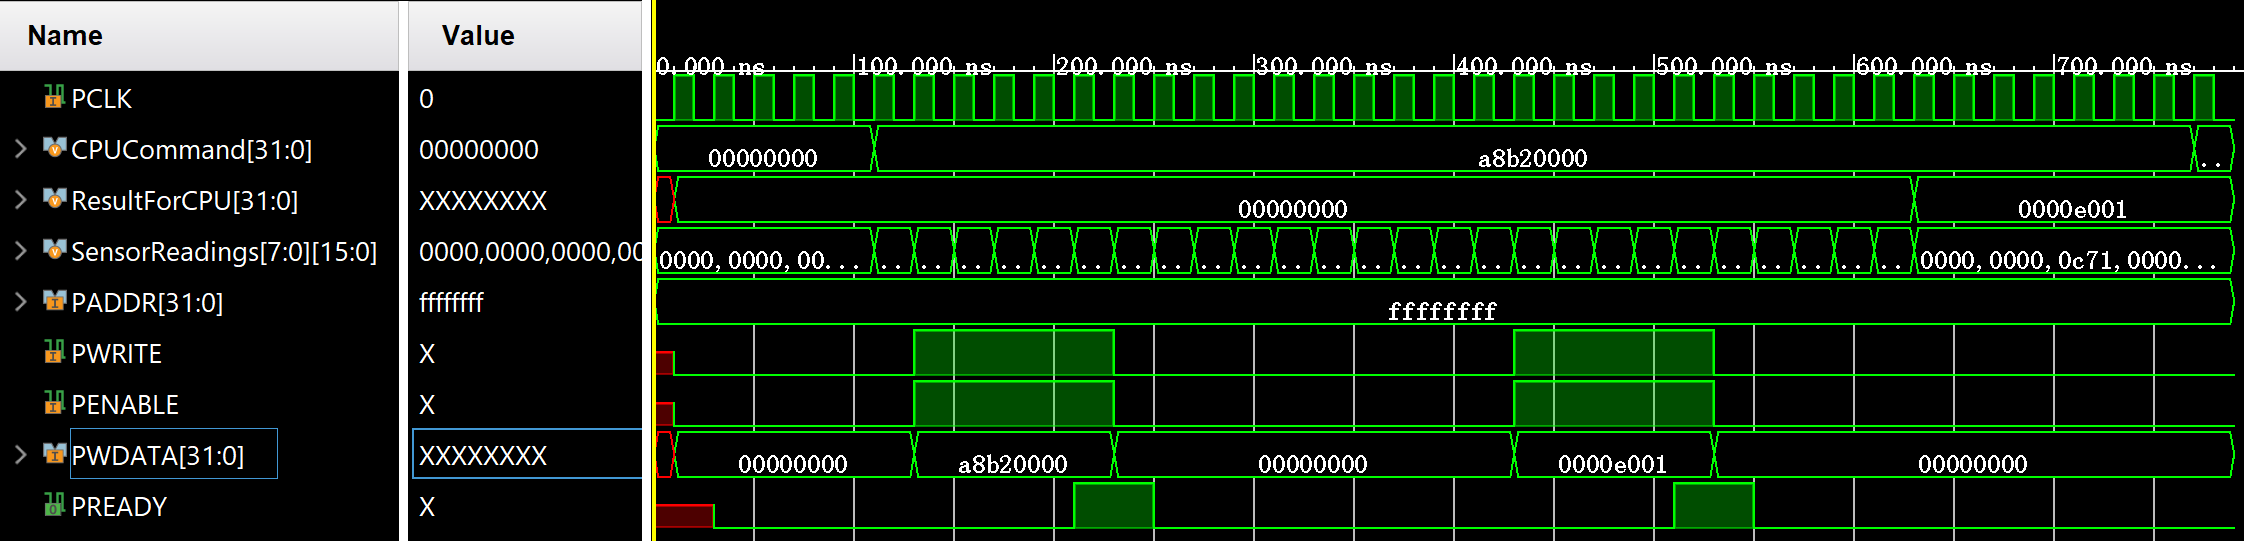
\includegraphics[width = 0.5\textwidth]{figures/error.png}
    \caption{Simulation waveform of an error case.}
    \label{fig:error}
\end{figure}

\subsection{APB SVA}
The simulation waveforms presented earlier also include APB signals. From the waveforms it can be seen that the toggling of these signals adheres to the APB protocol. All of the SVA properties defined in Section V have been successfully asserted. Figure \ref{fig:sva} is a snippet of the console messages during simulation. It shows a successful assertion and also a transaction captured by the UVM Monitor whose check passed in the Scoreboard.
\begin{figure*}[h!]
    \centering
    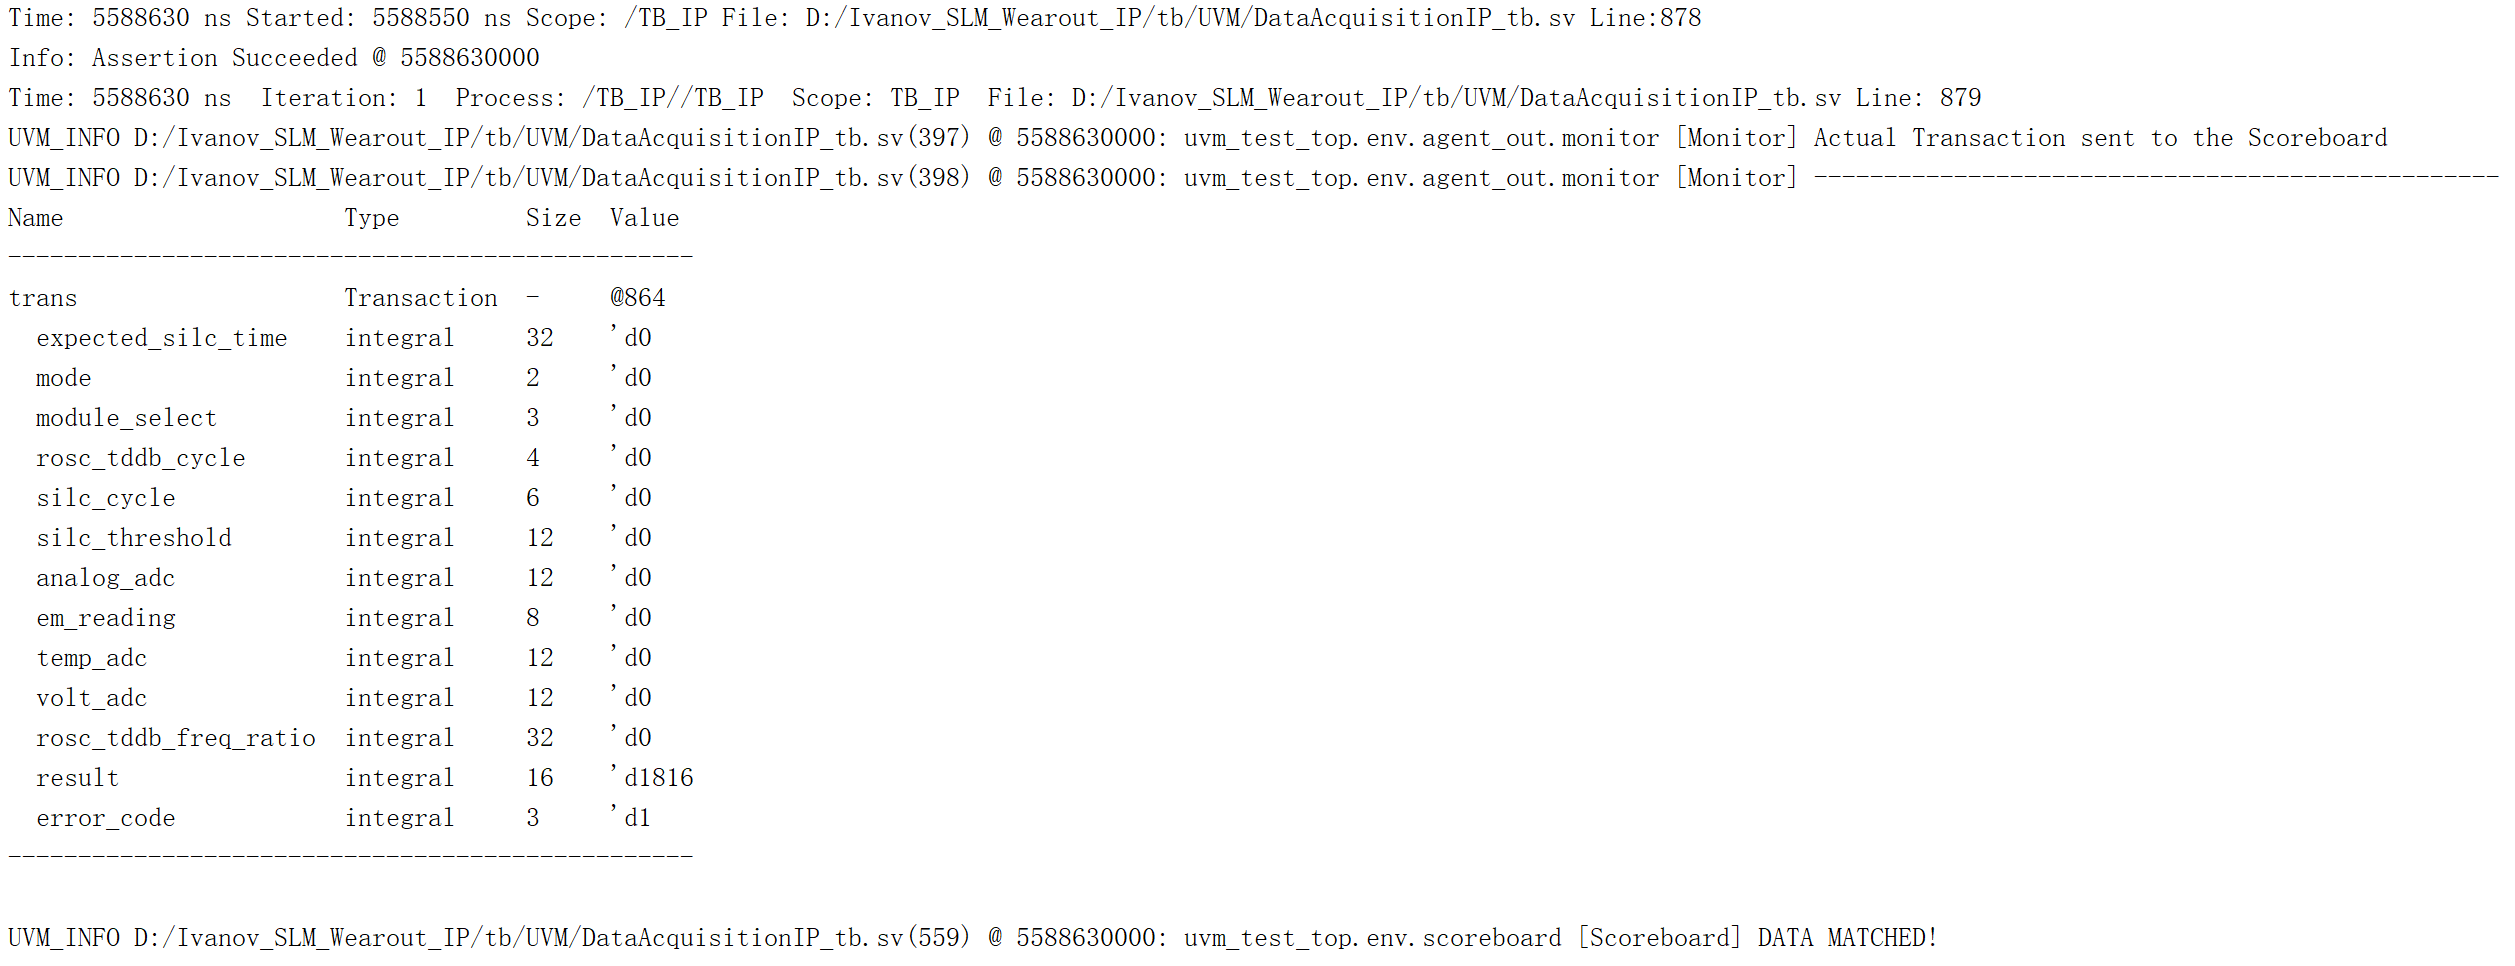
\includegraphics[width = \textwidth]{figures/sva.png}
    \caption{Console snippet during simulation.}
    \label{fig:sva}
\end{figure*}

\subsection{Functional Coverage}
100\% functional coverage has been achieved for both the module- and the IP-level verification. Figure \ref{fig:coverage} presents the IP's coverage report. The total coverage (left) and some of the coverpoints (right) are shown.
\begin{figure*}[h!]
    \centering
    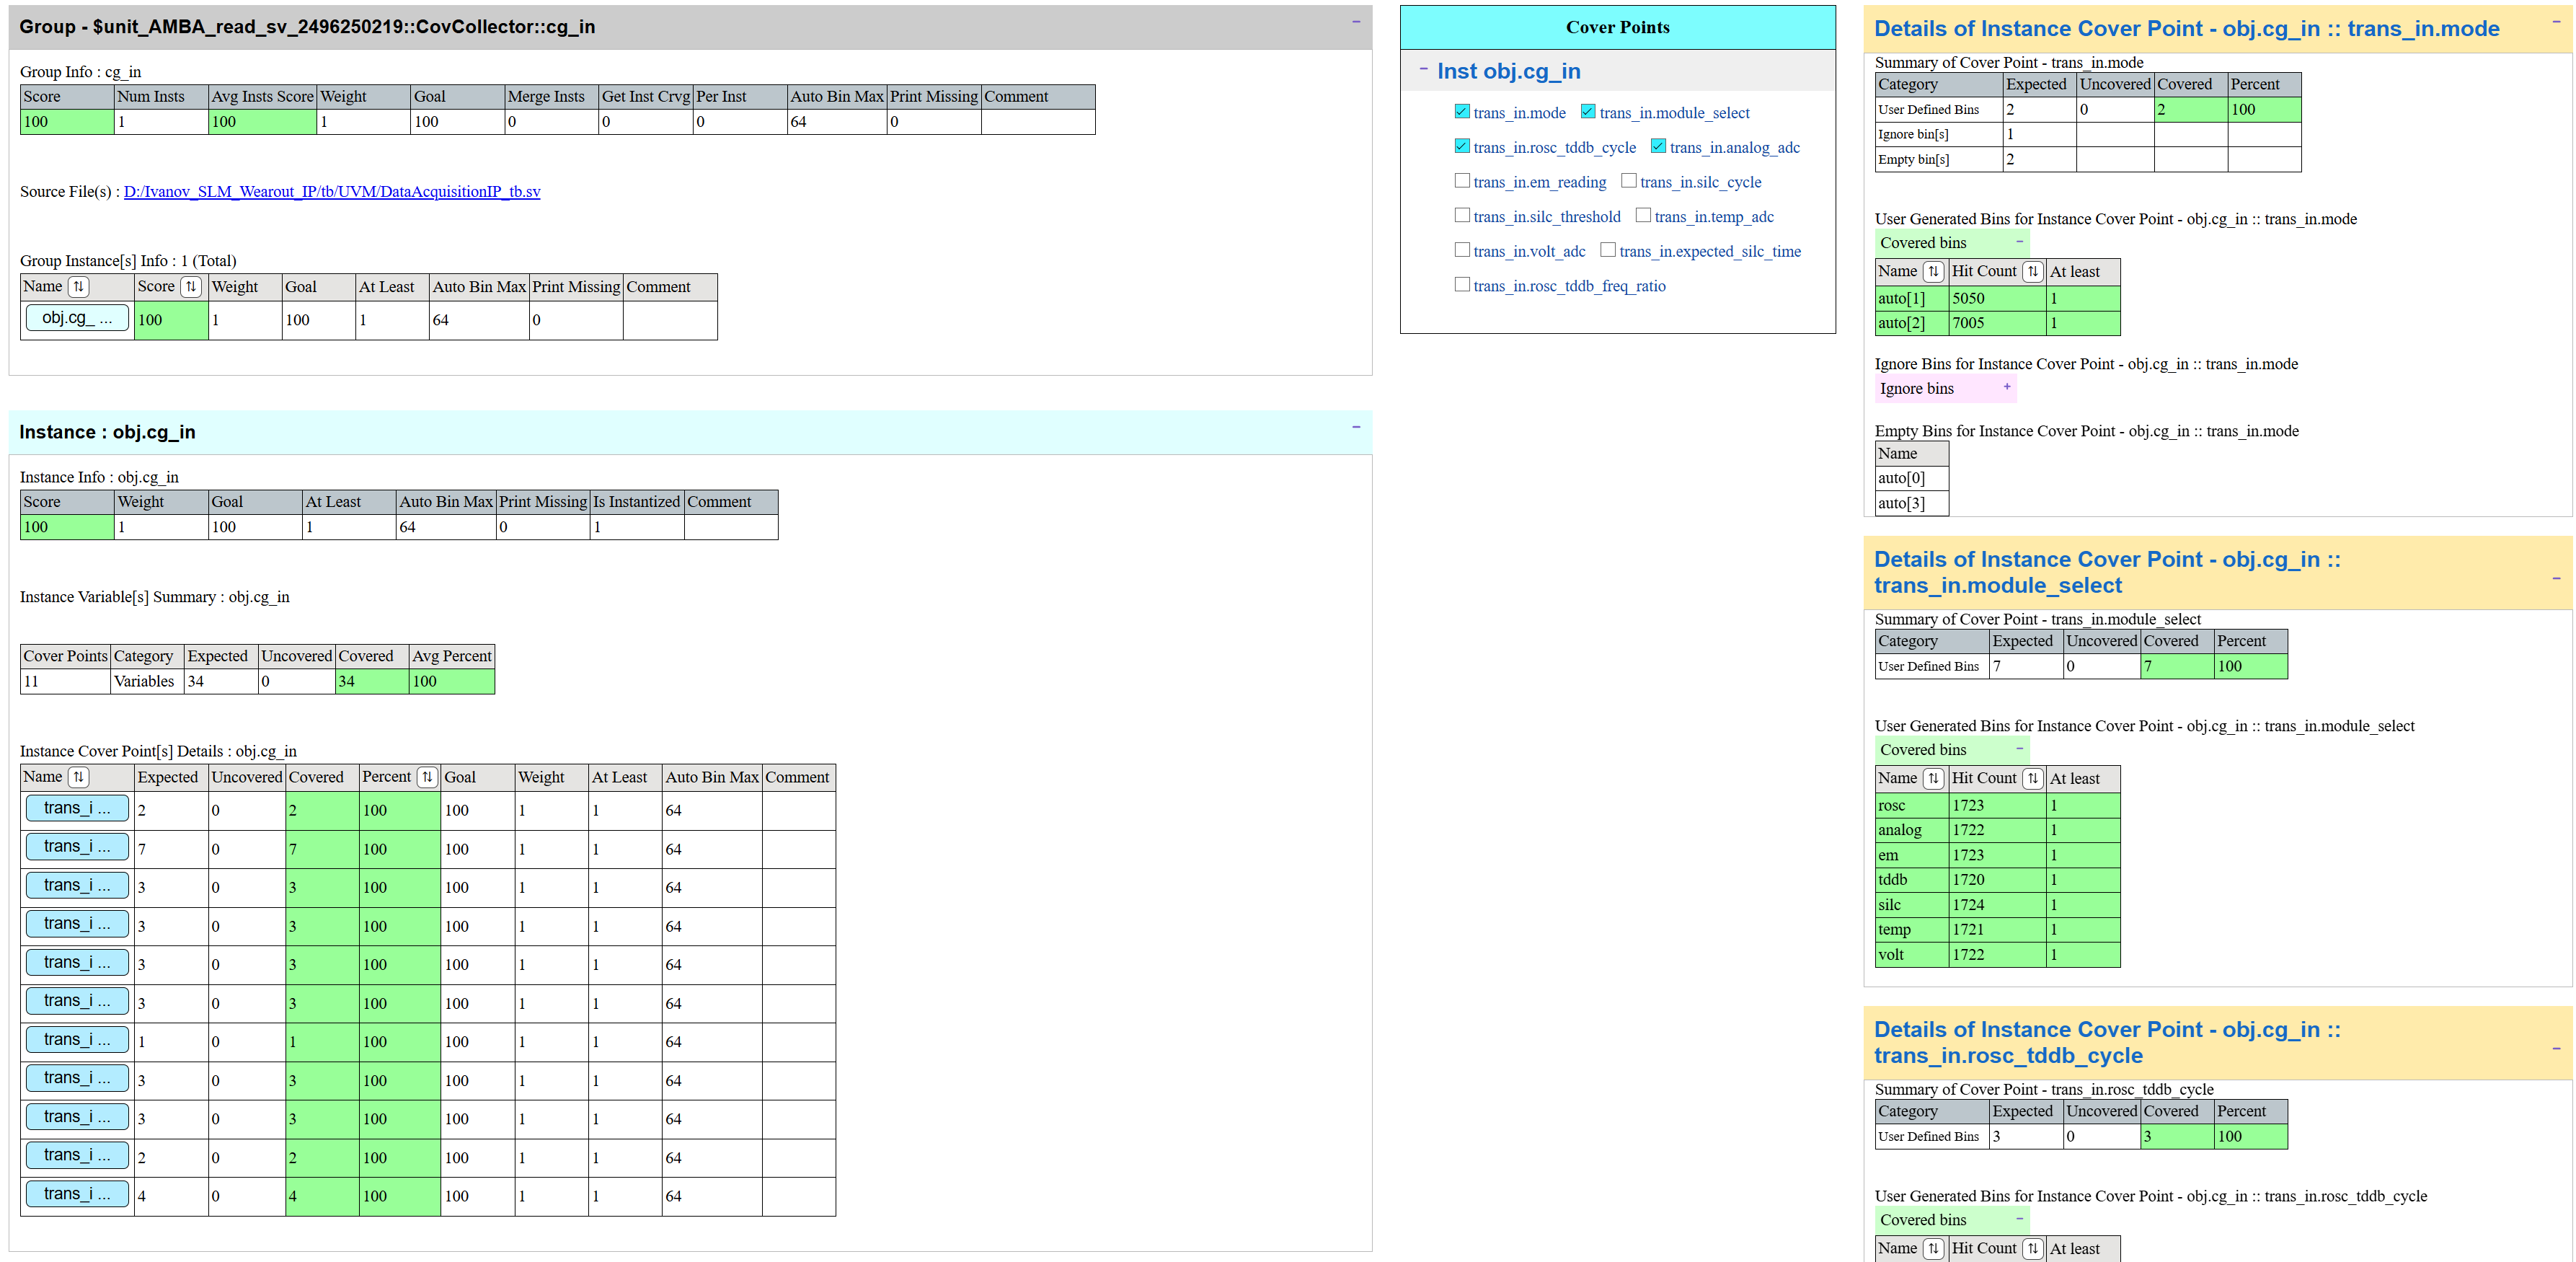
\includegraphics[width = \textwidth]{figures/coverage.png}
    \caption{Functional coverage report.}
    \label{fig:coverage}
\end{figure*}

\section{Conclusion}
An SLM wear-out monitoring IP with an AMBA APB interface has been successfully verified in this project. The proposed UVM testbenches could generate constrained random stimuli to achieve 100\% functional coverage. Such finding has proven the effectiveness of using UVM to conduct functional coverage-driven verifications as well as the practicality of using SVA for protocol verification. Similar verification methodology can be used for other designs with similar architecture.

\bibliographystyle{IEEEtran}
\bibliography{bibliography}

\end{document}
